\section{Introduction}
% WHERE: application in HRI
Robots operating in unstructured, dynamic environments must balance adapting the path to the surroundings and following a desired motion. In human-robot collaboration, they must efficiently complete their tasks while ensuring safe compliance in the presence of potential collisions.

% Fast control -> closed form DS
Velocity adjustments based on real-time sensory information are essential in complex and dynamic environments. Achieving this necessitates algorithms that are easily configurable and capable of rapid evaluation. As such, closed-form control laws eliminate the need for frequent replanning. Dynamical Systems (DS) is a valuable framework for representing such desired motion \cite{huber2019avoidance} where the behavior of the desired first-order DS is approximated through suitable controllers. 

% Compliance [Stay Reactive]
Most widely used robotic systems consist of rigid materials. Consequently, the interaction of these robotic systems with the surroundings leads to abrupt energy transfers, posing the risk of damage to the robot and its environment. However, modern robotic platforms are equipped with force and torque sensing capabilities that enable precise control over the forces exerted by the robot.
However, integrating these sensors makes the feedback controller more complex. The robot must achieve its designated position by following a desired velocity profile while remaining compliant with interaction forces. The control problem of balancing position, velocity, and force constraints is addressed by \textit{impedance controllers} \iflong
\parencite{takegaki1981new, hogan1984impedance} \else \parencite{hogan1985impedance}\fi.

% Ensure Obstacle Avoidance
Obstacle avoidance is fundamental to motion control, with reactive approaches capable of handling dynamic and intricate environments \parencite{huber2019avoidance}. The controller should remain compliant in free space while adhering to the desired motion when getting close to the obstacle. Furthermore, when encountering surfaces like fragile glass on a table, the controller must adopt stiffness to prevent a collision, yet it should be compliant when interacting with an operator (Fig.~\ref{fig:table_avoidance_with_obstacle}).

\begin{figure}
\centerline{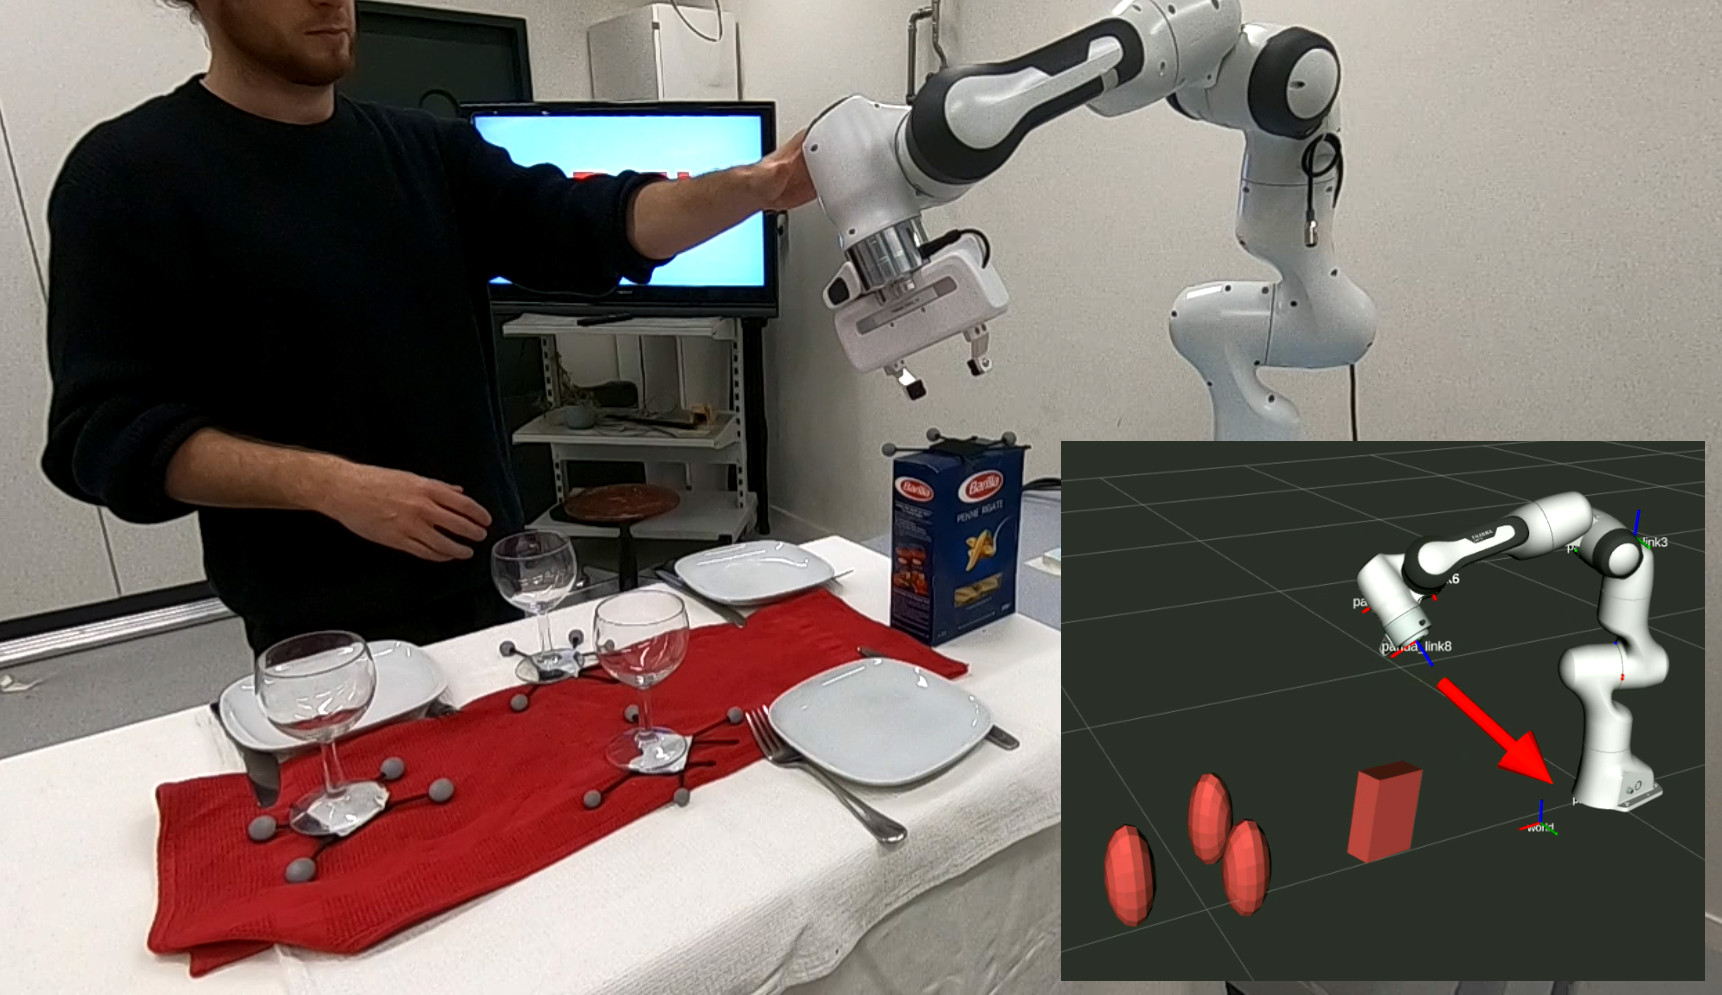
\includegraphics[width=.7\columnwidth]{figures/robot_arm_table_avoidance}}
\caption{
The proposed passive obstacle-aware controller lets the robot absorb external disturbances while ensuring collision avoidance. 
While tipping over the closed pasta box on this dinner table setup might be acceptable. Yet, the delicate wine glasses demand careful handling to prevent breakage.
}
\label{fig:table_avoidance_with_obstacle}
\end{figure}

This work introduces a novel approach incorporating dynamic obstacle avoidance using DS and variable impedance control, enhancing adaptability, reactivity, and safety in robotic movements. It empowers robots to navigate complex environments, proactively avoiding collisions and rejecting disturbances. Our approach is evaluated through \iflong simulations and \fi an implementation on a 7-degree-of-freedom (7DoF) robot arm, demonstrating robust and safe control in real-world scenarios.

